\chapter{Addestramento rete neurale}\label{addestramento-rete-neurale}


Come già menzionato nei capitoli precedenti l’idea è quella di allenare una  CNN per la classificazione dei frame di una laringoscopia attravero il transfer learning impiegando la tecnica del
fine-tuning nelle due varianti (One Round Tuning e Two Round Tuning)  su una rete pre-allenata chiamata AlexNet.

\section{AlexNet}\label{alexnet}
AlexNet è la rete che ha rivoluzionato la computer vision nel 2012, essa è una CNN sviluppada
da Goffrey Hinton e Alex Krizhevsky dell’università di Toronto vince (con ampio margine)
l’ImageNet challenge: object classification and detection su milioni di immagini e 1000 classi.

La rete AlexNet è organizzata nel seguente modo: costituita da 8 livelli di cui 5 di \gls{convoluzione} e 3 \gls{fully-connected}, utilizza la funzione
di attivazione \gls{ReLu}, con dimensione delle immagini in input è di \(227\times 227\), l'architettura completa con le dimensioni dei layer di \gls{convoluzione} è illustrata in \cref{fig:alexnet}\cite{alexnet}.  

\begin{figure}[ht]
    \centering
    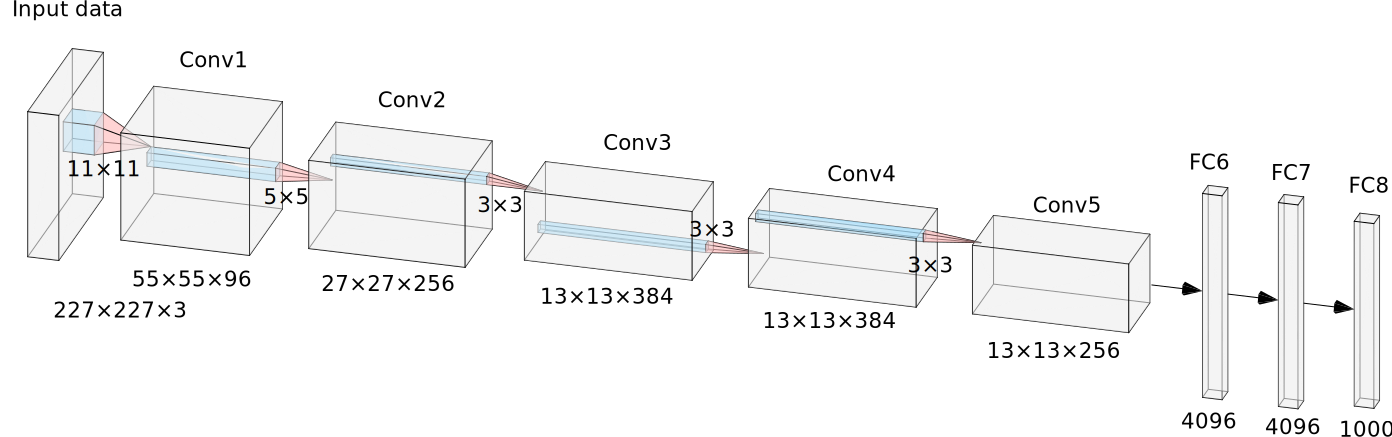
\includegraphics[width=0.7\textwidth]{addestramento-rete-neurale/alexnet.png}
    \caption{Architettura della CNN AlexNet}
    \label{fig:alexnet}
\end{figure}

La rete AlexNet utilizzata è già allenata per il riconoscimento di 1000 classi di soggetti (mele, gatti, tastiere, telefoni, ecc.) su un dataset di oltre 1 milione di pattern presi dal database ImageNet\cite{alexnet}.

\section{Allenamento 1R}\label{allenamento-1r}

La sperimentazione inizia con l'allenamento della CNN in con un fine-tuning standard e classico, nel senso rimpiazzo gli ultimi 3 layer e poi rialleno la rete. È da prestare attenzione a i vali iperparametri, come Learning Rate e MiniBatch Size.

\section{Allenamento 2R}\label{allenamento-2r}
